% Этот шаблон документа разработан в 2014 году
% Данилом Фёдоровых (danil@fedorovykh.ru) 
% для использования в курсе 
% <<Документы и презентации в \LaTeX>>, записанном НИУ ВШЭ
% для Coursera.org: http://coursera.org/course/latex .
% Исходная версия шаблона --- 
% https://www.writelatex.com/coursera/latex/3.2

\documentclass[a4paper,12pt]{article}

%%% Работа с русским языком
\usepackage{cmap}					% поиск в PDF
\usepackage{mathtext} 				% русские буквы в формулах
\usepackage[T2A]{fontenc}			% кодировка
\usepackage[utf8]{inputenc}			% кодировка исходного текста
\usepackage[english,russian]{babel}	% локализация и переносы

%%% Дополнительная работа с математикой
\usepackage{amsmath,amsfonts,amssymb,amsthm,mathtools} % AMS
\usepackage{icomma} % "Умная" запятая: $0,2$ --- число, $0, 2$ --- перечисление

%% Номера формул
%\mathtoolsset{showonlyrefs=true} % Показывать номера только у тех формул, на которые есть \eqref{} в тексте.
%\usepackage{leqno} % Нумерация формул слева

%% Свои команды
\DeclareMathOperator{\sgn}{\mathop{sgn}}

%% Перенос знаков в формулах (по Львовскому)
\newcommand*{\hm}[1]{#1\nobreak\discretionary{}
	{\hbox{$\mathsurround=0pt #1$}}{}}

%%% Работа с картинками
\usepackage{graphicx}  % Для вставки рисунков
\graphicspath{{images/}{images2/}}  % папки с картинками
\setlength\fboxsep{3pt} % Отступ рамки \fbox{} от рисунка
\setlength\fboxrule{1pt} % Толщина линий рамки \fbox{}
\usepackage{wrapfig} % Обтекание рисунков текстом

%%% Работа с таблицами
\usepackage{array,tabularx,tabulary,booktabs} % Дополнительная работа с таблицами
\usepackage{longtable}  % Длинные таблицы
\usepackage{multirow} % Слияние строк в таблице

%%% Теоремы
\theoremstyle{plain} % Это стиль по умолчанию, его можно не переопределять.
\newtheorem{theorem}{Теорема}[section]
\newtheorem{proposition}[theorem]{Утверждение}

\theoremstyle{definition} % "Определение"
\newtheorem{corollary}{Следствие}[theorem]
\newtheorem{problem}{Задача}[section]

\theoremstyle{remark} % "Примечание"
\newtheorem*{nonum}{Решение}

%%% Программирование
\usepackage{etoolbox} % логические операторы

%%% Страница
\usepackage{extsizes} % Возможность сделать 14-й шрифт
\usepackage{geometry} % Простой способ задавать поля
\geometry{top=25mm}
\geometry{bottom=35mm}
\geometry{left=35mm}
\geometry{right=20mm}
%

\usepackage{fancyhdr} % Колонтитулы
\pagestyle{fancy}
%\renewcommand{\headrulewidth}{0mm}  % Толщина линейки, отчеркивающей верхний колонтитул
%\lfoot{Нижний левый}
%\rfoot{Нижний правый}
%\rhead{}
%\chead{Верхний в центре}
\lhead{}
% \cfoot{Нижний в центре} % По умолчанию здесь номер страницы

\usepackage{setspace} % Интерлиньяж
%\onehalfspacing % Интерлиньяж 1.5
%\doublespacing % Интерлиньяж 2
%\singlespacing % Интерлиньяж 1

\usepackage{lastpage} % Узнать, сколько всего страниц в документе.

\usepackage{soul} % Модификаторы начертания

\usepackage{indentfirst} % Красная строка

\usepackage{soulutf8} % Модификаторы начертания

%\usepackage{hyperref}
%\usepackage[usenames,dvipsnames,svgnames,table,rgb]{xcolor}
%\hypersetup{				% Гиперссылки
%	unicode=true,           % русские буквы в раздела PDF
%	pdftitle={Заголовок},   % Заголовок
%	pdfsubject={Тема},      % Тема
%	pdfcreator={Создатель}, % Создатель
%	pdfproducer={Производитель}, % Производитель
%	pdfkeywords={keyword1} {key2} {key3}, % Ключевые слова
%	colorlinks=true,       	% false: ссылки в рамках; true: цветные ссылки
%	linkcolor=red,          % внутренние ссылки
%	citecolor=green,        % на библиографию
%	filecolor=magenta,      % на файлы
%	urlcolor=cyan           % на URL
%}

%\renewcommand{\familydefault}{\sfdefault} % Начертание шрифта

\usepackage{multicol} % Несколько колонок

\author{\LaTeX{} в Вышке}
\title{3.2 Оформление документа в целом}
\date{\today}

\begin{document} % конец преамбулы, начало документа
\thispagestyle{empty}
\begin{center}
	\textit{Федеральное государственное автономное образовательное\\ учреждение высшего образования }
	\vspace{0.5ex}
	
	\textbf{«Московский физико-технический институт\\ (национальный исследовательский университет)»}
\end{center}
\vspace{10ex}
%\begin{flushright}
%	\noindent
%	\textit{Фамилия Имя Отчество}
%	\\
%	\textit{студент факультета экономики \\(группа 211И)}
%\end{flushright}
\begin{center}
	\vspace{13ex}
	\so{\textbf{Лабораторная работа №1.3.3}}
	\vspace{1ex}
	
	по курсу общей физики
	
	
	на тему:
	
	\textbf{\textit{<<Определение вязкости воздуха\\ по скорости течения через тонкие трубки>>}}
	\vspace{30ex}
	\begin{flushright}
		\noindent
		\textit{Работу выполнил:}
		\\
		\textit{Баринов Леонид \\(группа Б02-827)}
	\end{flushright}
	\vfill
	Долгопрудный \\2019 год
\end{center}

\newpage
\setcounter{page}{1}
\section{Аннотация}
В работе будет экспериментально выявлен участок сформированного течения, определены режимы ламинарного и турбулентного течения, определено число Рейнольдса.
\section{Теоритические сведения}
\subsection{Формула Пуазейля}
Уравнение Бернулли:
\begin{equation}
\frac{\upsilon^2}{2}+gh_1+\frac{p}{\rho} = const
\end{equation}

В соответствии с уравнением Бернулли при стационарном течении по прямолинейной горизонтальной трубе постоянного сечения давление жидкости должно быть одним и тем же по всей длине трубы. В действительности, однако, давление жидкости в трубе падает в направлении течения. Для обеспечения стационарности течения необходимо поддерживать на концах трубы постоянную разность давлений, уравновешивающую силы внутреннего трения, которые возникают при течении жидкости.

Сила трения между слоями жидкости зависит от изменения скорости в перпендикулярном потоку направлении (закон Ньютона для вязкой жидкости):
\begin{equation}
F = S\eta\frac{d\upsilon_x}{dy}
\end{equation}

Для вывода формулу Пуазейля рассмотрим следующую физическую модель. Пусть вязкая несжимаемая жидкость течет вдоль прямолинейной цилиндрической трубы радиусом $R$. Координатную ось $x$ направим вдоль оси трубы в сторону течения. Выделим в трубе произвольную бесконечно короткую цилиндрическую часть длиной $dx$ и радиусом $r$ (рис. 1).

\begin{wrapfigure}{r}{0.3333\linewidth}
\label{1}
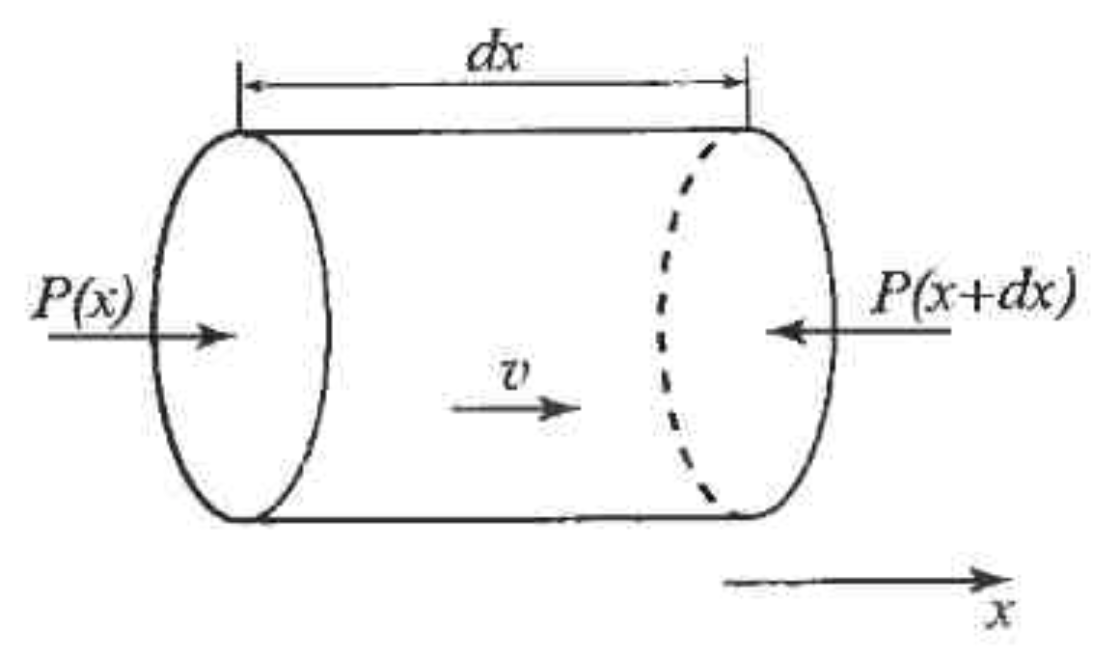
\includegraphics[width=\linewidth]{1}
\caption{К выводу формулы Пуазейля}
\end{wrapfigure}
На боковую поверхность выделенного цилиндра в направлении, противоположном движению, действует касательная сила вязкого трения:
\begin{equation}
dF = 2\pi r\eta\frac{d\upsilon}{dr}dx
\end{equation}

На основания цилиндра в направлении движения действует сила разности давлений:
\begin{equation}
dF_1 = \pi r^2 (P(x)-P(x+dx)) = -\pi r^2\frac{dP}{dx}dx
\end{equation}

При стационарном течении ускорение выделенного объема жидкости должно быть равно нулю. Следовательно:
\begin{equation}
\begin{aligned}
dF + dF_1 = 0\\
2\eta\frac{d\upsilon}{dr} = r\frac{dP}{dx}
\end{aligned}
\end{equation}

Скорость $\upsilon$ не зависит от $x$, следовательно производная $dP/dx$ должна быть постоянной, равной
\[\frac{P_2-P_1}{l}\]
где $P_1$ -- давление на входе трубы, $P_2$ -- давление на выходе трубы. В результате имеем
\begin{equation}
\frac{d\upsilon}{dr} = -\frac{P_1-P_2}{2\eta l}r
\end{equation}
Интегрируя при условии прилипании жидкости к стенке трубы $\upsilon(R) = 0$:
\begin{equation}
\upsilon = \frac{P_1 - P_2}{4\eta l}(R^2-r^2)
\end{equation}
Скорость $\upsilon$ максимальна на оси трубы, где она достигает значения
\[\upsilon_0 = \frac{P_1 - P_2}{4\eta l}R^2\] 
Определим расход жидкости:
\[Q = \pi\rho\frac{P_1-P_2}{2\eta l}\int\limits_{0}^{R}(R^2 - r^2)rdr \]
\begin{equation}
\label{Pus}
Q = \pi\rho\frac{P_1-P_2}{8\eta l}R^4
\end{equation}
Формулу \eqref{Pus} принято называть формулой Пуазейля

На практике расход жидкости удобно измерять в единицах объема жидкости, протекающей в единицу времени через поперечное сечение. Формула \eqref{Pus} примет вид:
\begin{equation}
Q_V = \frac{\pi R^4}{8\eta l}(P_1 - P_2)
\end{equation}
\subsection{Число Рейнольдса}
Число Рейнольдса (Re) -- это единственная безразмерная величина, которую можно составить из параметров $\rho, U, l, \eta$.\\
Здесь $l$ -- характерная длина, $U$ -- характерная скорость течения.
\begin{equation}
\text{Re} = \frac{\rho U l}{\eta}
\end{equation}

Число Рейнольдса отражает свойство подобия гидродинамических течений: при изменении параметров жидкости и тела, но при сохранении значения Re характер течения не меняется.

\[\frac{E_\text{к}}{A_\text{тр}}\sim \text{Re}\]

Таким образом, если вязкость мала, то Re $\gg 1$ и доминируют инерционные эффекты, жидкость близка к идеальной. Если же вязкость велика, то Re $\ll 1$ и доминируют эффекты вязкости.

В гладких трубах круглого сечения переход от ламинарного движения к турбулентному происходит при Re $\approx 1000$.

Характерное для ламинарного течения параболическое распределение скоростей устанавливается на некотором расстоянии $a$ от входа в трубку, которое зависит от радиуса трубки $r$  и числа Рейнольдса по формуле:
\begin{equation}
a \approx 0,2r \cdot \text{Re}
\end{equation}
\section{Оборудование}
В работе используются: металлические трубки, укрепленные на горизонтальной подставке, газовый счетчик, микроманометр типа ММН, стеклянная U-образная трубка, секундомер.
\subsection{Экспериментальная установка}
\begin{figure}[h]
	\begin{center}
		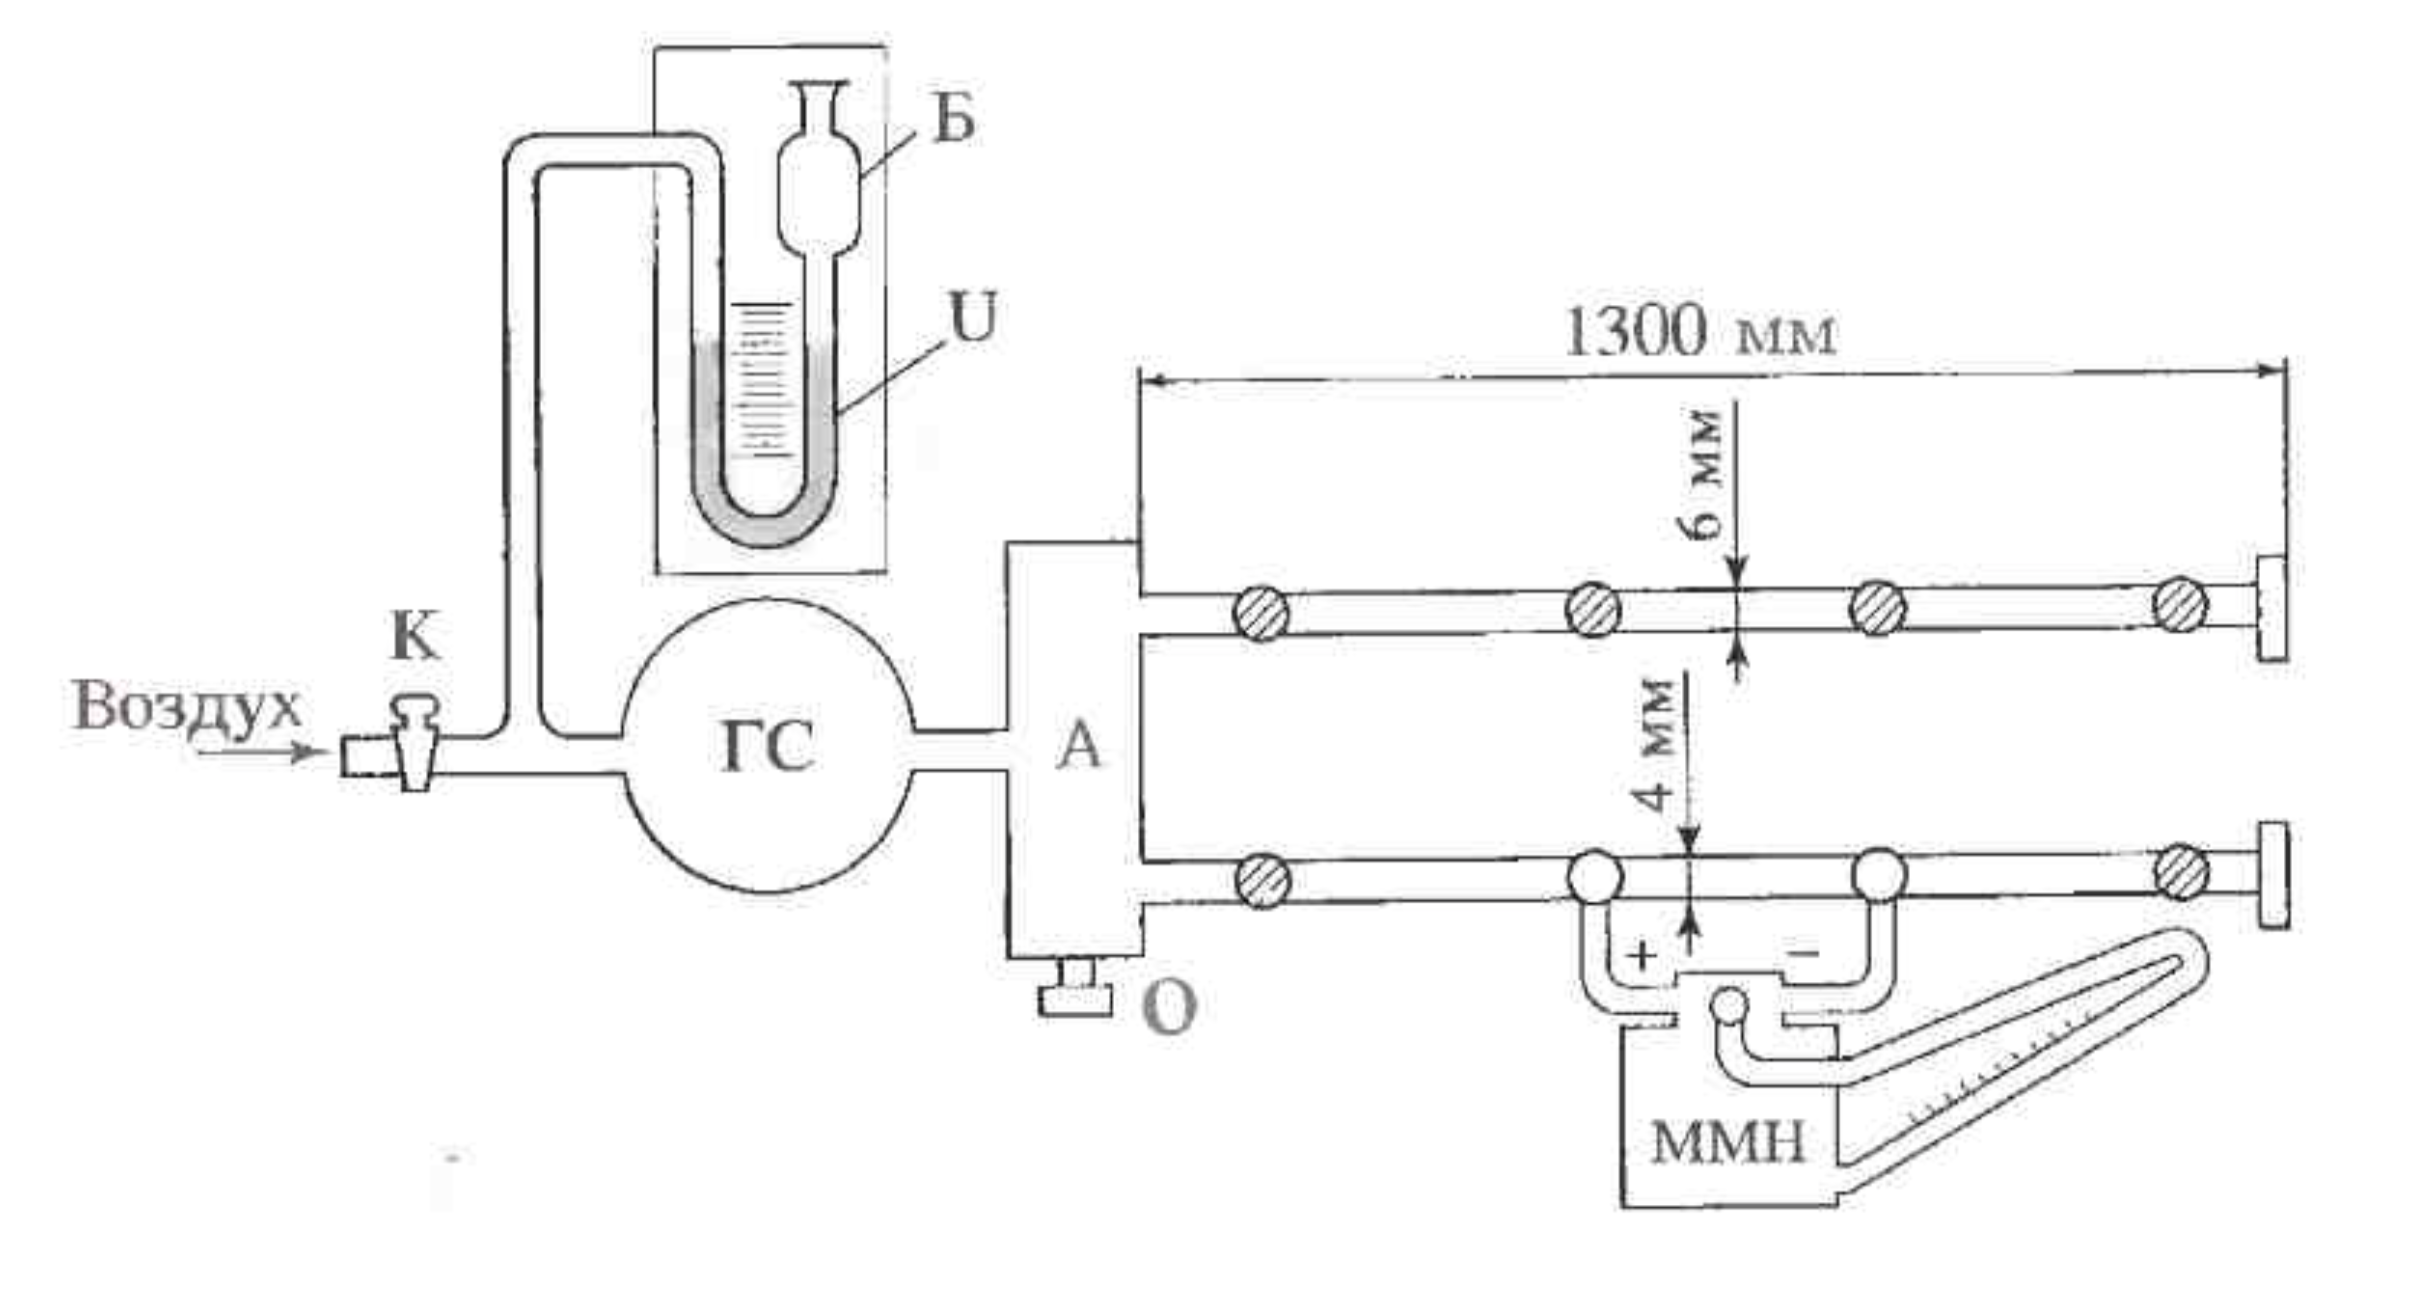
\includegraphics[width=\linewidth]{2}
		\caption{Схема установки для определения вязкости воздуха}
	\end{center}
\end{figure}
\noindent ГС -- газовый счетчик;\\
U -- образная трубка, наполовину заполненная водой\\
Б -- защитный баллон, который предупреждает о высоком давлении\\
К -- кран, для регулировки подачи воздуха\\
А -- резервуар, к которому припаянные тонкие металлические трубки\\
ММН -- микроманометр
\subsection{Микроманометр типа ММН}
\begin{figure}[h]
	\begin{center}
		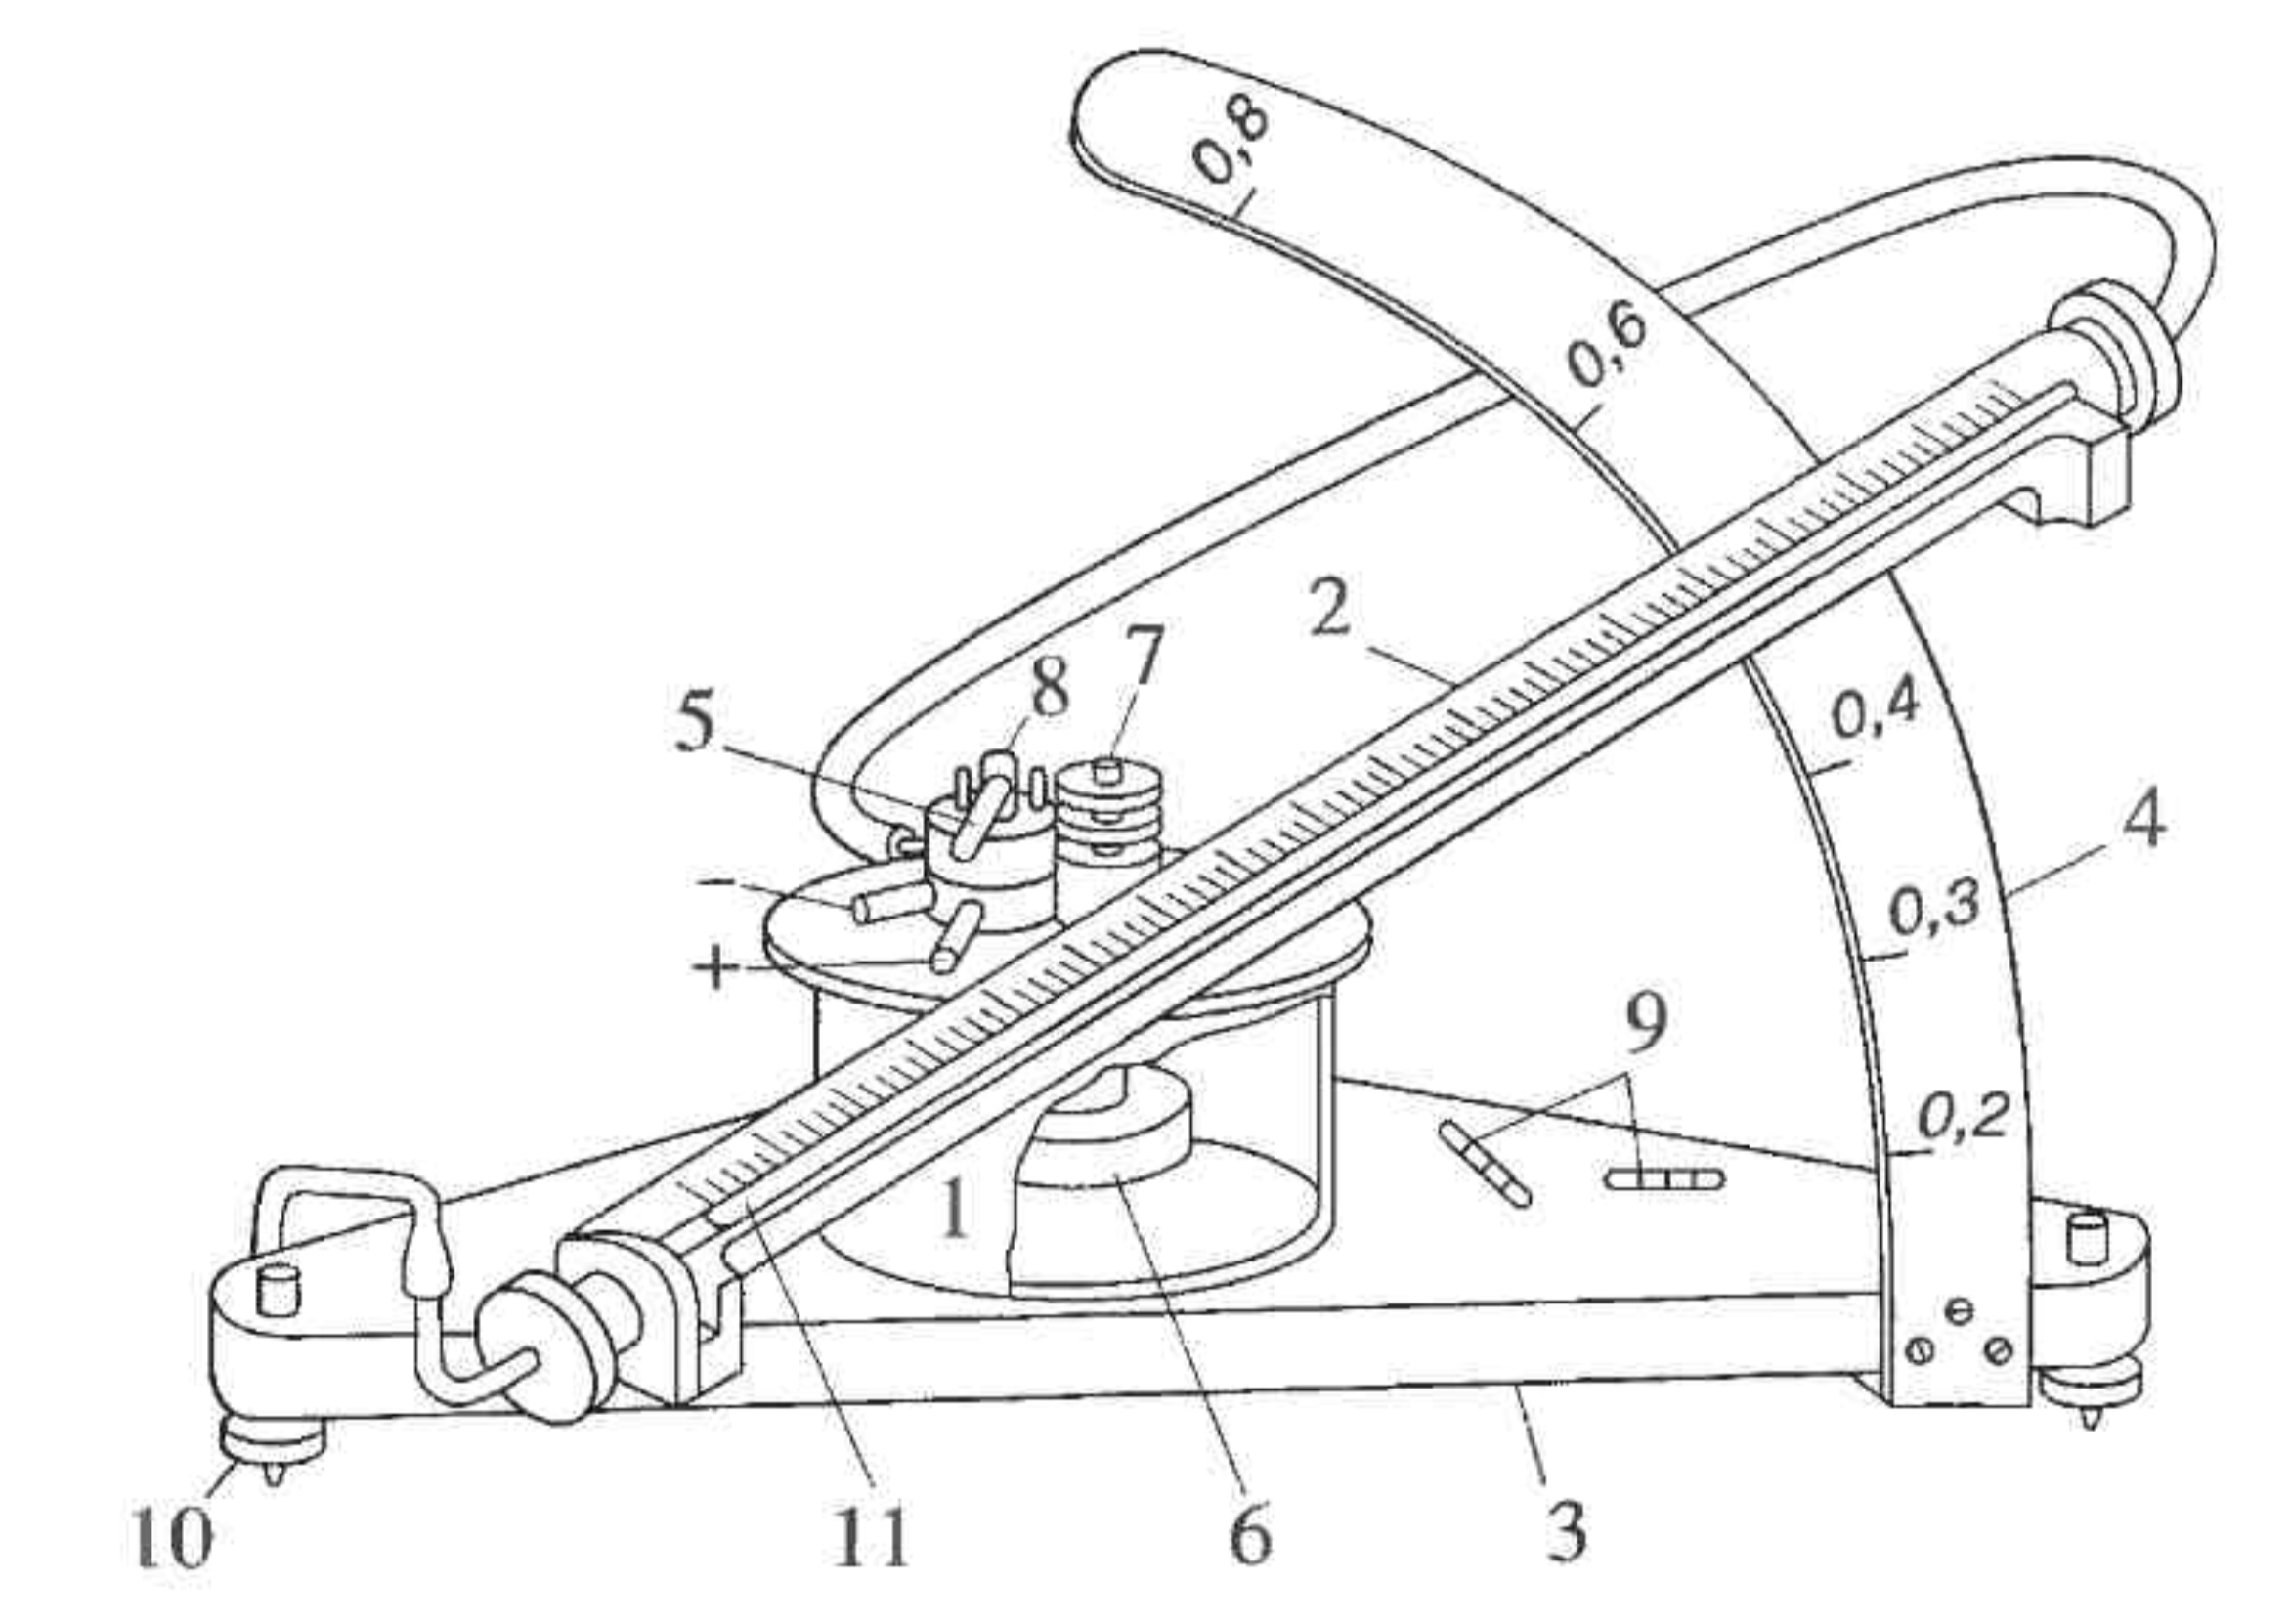
\includegraphics[width=0.5\linewidth]{3}
		\caption{Микрометрический манометр типа ММН}
	\end{center}
\end{figure}
\begin{itemize}

\item Числа 0,2; 0,3; 0,4; 0,6; и 0,8, нанесенные на стойке 4, обозначают коэффициент, на который должны быть умножены показания манометра при данном наклоне, для получения давления в миллиметрах водяного столба.
\item Рабочей жидкостью является этиловый спирт.
\item Установка меникса жидкости на нуль шкалы производится путем изменения уровня спирта в сосуде 1 с помощью цилиндра 6.
\item Глубина погружения цилиндра в спирт регулируется винтом 7.
\item Микроманометр снабжен двумя уровнями 9, расположенными на плите 3 перпендикулярно один другому. Установка прибора по уровням производится двумя регулировочными ножками 10.
\item Трехходовой кран 8, который имеет два рабочих положения -- <<0>> и <<+>>. В положении <<0>> мениск жидкости устанавливается на ноль. В положении <<+>> производятся рабочие измерения. Перевод из положения <<0>> в положение <<+>> и наоборот осуществляется с помощью рычажка 5.
\item Погрешность микроманометра в положении 0,2: $\Delta p = 0,04 \ \text{мм вод. ст.}$
\end{itemize}
 \subsection{Газовый счетчик}
 Газовый счетчик служит для измерения небольших количеств газа. Внешний вид его изображен на рис. 4.
 \begin{itemize}
 	\item Один оборот стрелки соотвествует 5 л газа, прошедшего через счетчик.
 	\item Газовый счетчик заливается водой до уровня, определяемого по водомерного устройству 1.
 	\item Трубка 2 для входа газа расположена сзади счетчика, а трубка 3 для выхода газа -- наверху счетчика.
 

 \begin{figure}[h]
 	\begin{center}
 		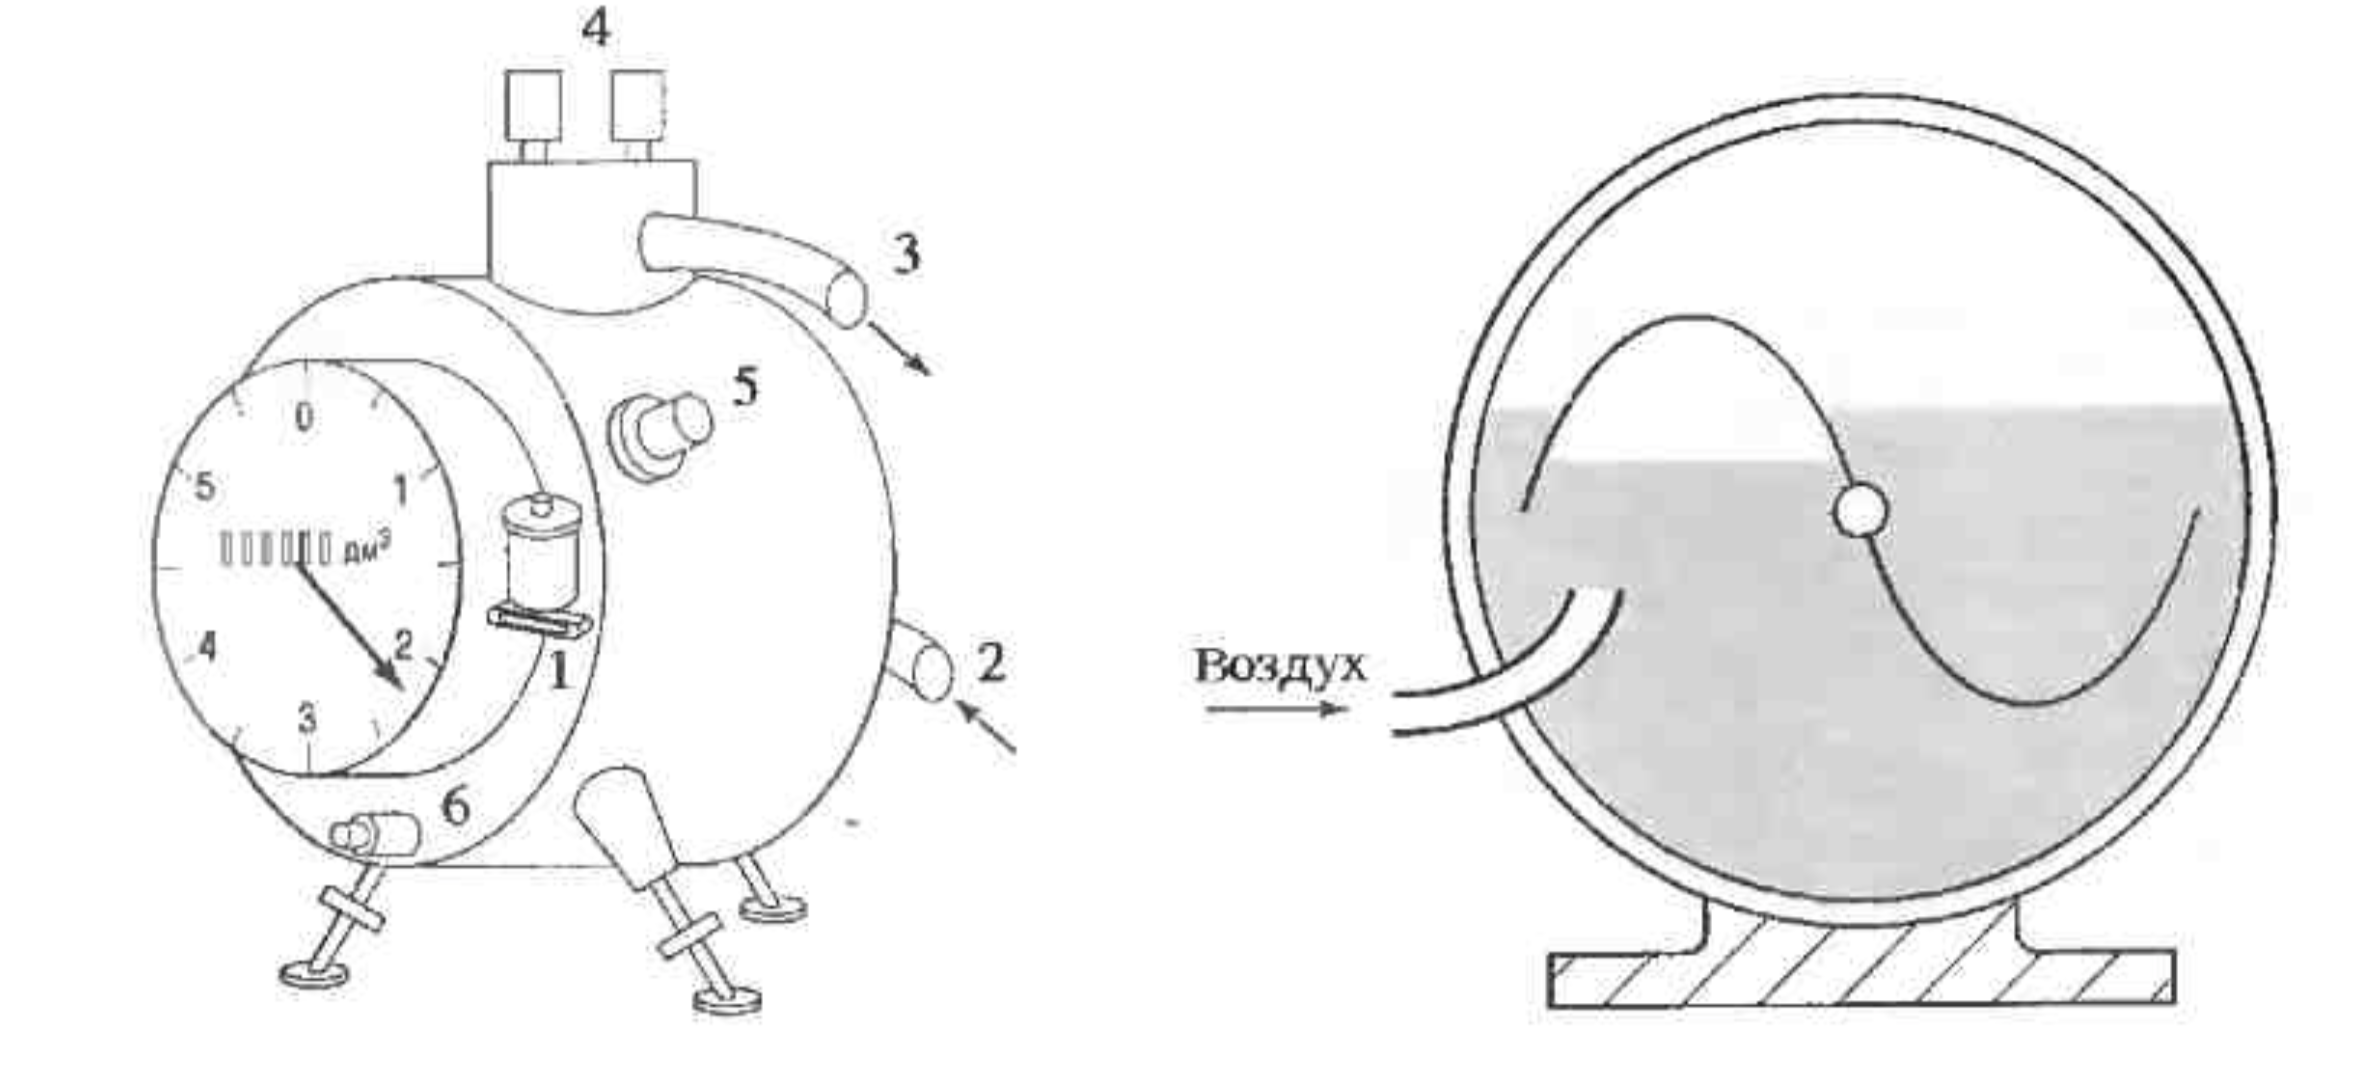
\includegraphics[width=0.5\linewidth]{4}
 		\caption{Газовый счетчик}
 	\end{center}
 \end{figure}
	\item Патрубки 4 предназначены для присоединения U-образного манометра, а патрубок 5 -- для установки термометра.
\item Кран 6 служит для слива воды.
\item Погрешность газового счетчика: $\Delta V = 0,02\ \text{л}$
\end{itemize}
\section{Результаты измерений и обработка результатов}
В работе будут использованы три трубки, диаметры которых указаны в Таблице 1. Оценим расстояния, на котором происходит формирование потока при ламинарном течении по формуле (11). Расчет проведем для Re $=1000$

\begin{table}[h]
	\begin{center}
	\begin{tabular}{|c|c|c|c|}
		\hline
		$d, \text{мм}$  & $\Delta d, \text{мм}$ & $a, мм$ &$\Delta a, \text{мм}$ \\ \hline
		3   & 0,01 & 300 & 1 \\ \hline
		4,1 & 0,05 & 410 & 5 \\ \hline
		5,8 & 0,05 & 580 & 5 \\ \hline
	\end{tabular}
\caption{Расстояние $a$, на котором будет происходит формирование потока при ламинарном течении}
\end{center}
\end{table}
\subsection{Измерение вязкости воздуха}
Снимем зависимость разности давлений $\Delta P$ от расхода воздуха $Q = \Delta V/ \Delta t$, при этом $\Delta V$ измеряется газовым счетчиком, а $\Delta t$ -- секундомером. Результаты занесем в Таблицу 2.
\begin{longtable}{|c|c|c|c|c|}
	\hline
$\text{№}$ &  $\Delta P, \text{мм вод. ст.}$  & $\Delta V, \text{л}$ & $\Delta t, \text{с}$ & $Q, \text{л/с}$        \\ \hline
	\endfirsthead
	\hline
	$\text{№}$ &  $\Delta P, \text{мм вод. ст.}$  & $\Delta V, \text{л}$ & $\Delta t, \text{с}$    &  $Q, \text{л/с}$     \\ \hline
	\endhead
	\hline
	\endfoot

	\endlastfoot

1  & 0,8  & 1   & 156,62 & 0,006 \\ \hline
2  & 1,8  & 1   & 67,34  & 0,015 \\ \hline
3  & 3    & 1   & 43     & 0,023 \\ \hline
4  & 4,2  & 1,1 & 32,88  & 0,033 \\ \hline
5  & 5,2  & 1,3 & 33,69  & 0,039 \\ \hline
6  & 6    & 1,4 & 30,56  & 0,046 \\ \hline
7  & 6,6  & 1,8 & 33,68  & 0,053 \\ \hline
8  & 8    & 1,9 & 32,31  & 0,059 \\ \hline
9  & 9    & 2,2 & 33,03  & 0,067 \\ \hline
10 & 10   & 2,5 & 33,43  & 0,075 \\ \hline
11 & 10,8 & 2,5 & 31,84  & 0,079 \\ \hline
12 & 12   & 3   & 34,6   & 0,087 \\ \hline
13 & 13   & 3   & 32,68  & 0,092 \\ \hline
14 & 14,2 & 3   & 31,41  & 0,096 \\ \hline
15 & 15,8 & 3,2 & 32,28  & 0,099 \\ \hline
16 & 18   & 3,5 & 33,53  & 0,104 \\ \hline
17 & 32,2 & 4,5 & 33,63  & 0,134 \\ \hline
18 & 43   & 5   & 32     & 0,156 \\ \hline
19 & 59   & 6   & 32,53  & 0,184 \\ \hline

\caption {Зависимость разности давлений $\Delta P$ от расхода воздуха $Q$}
\end{longtable}
По полученным данным построим график зависимости $\Delta P$ от $Q$ (Рис. 5)
\begin{figure}[!h]
	\begin{center}
		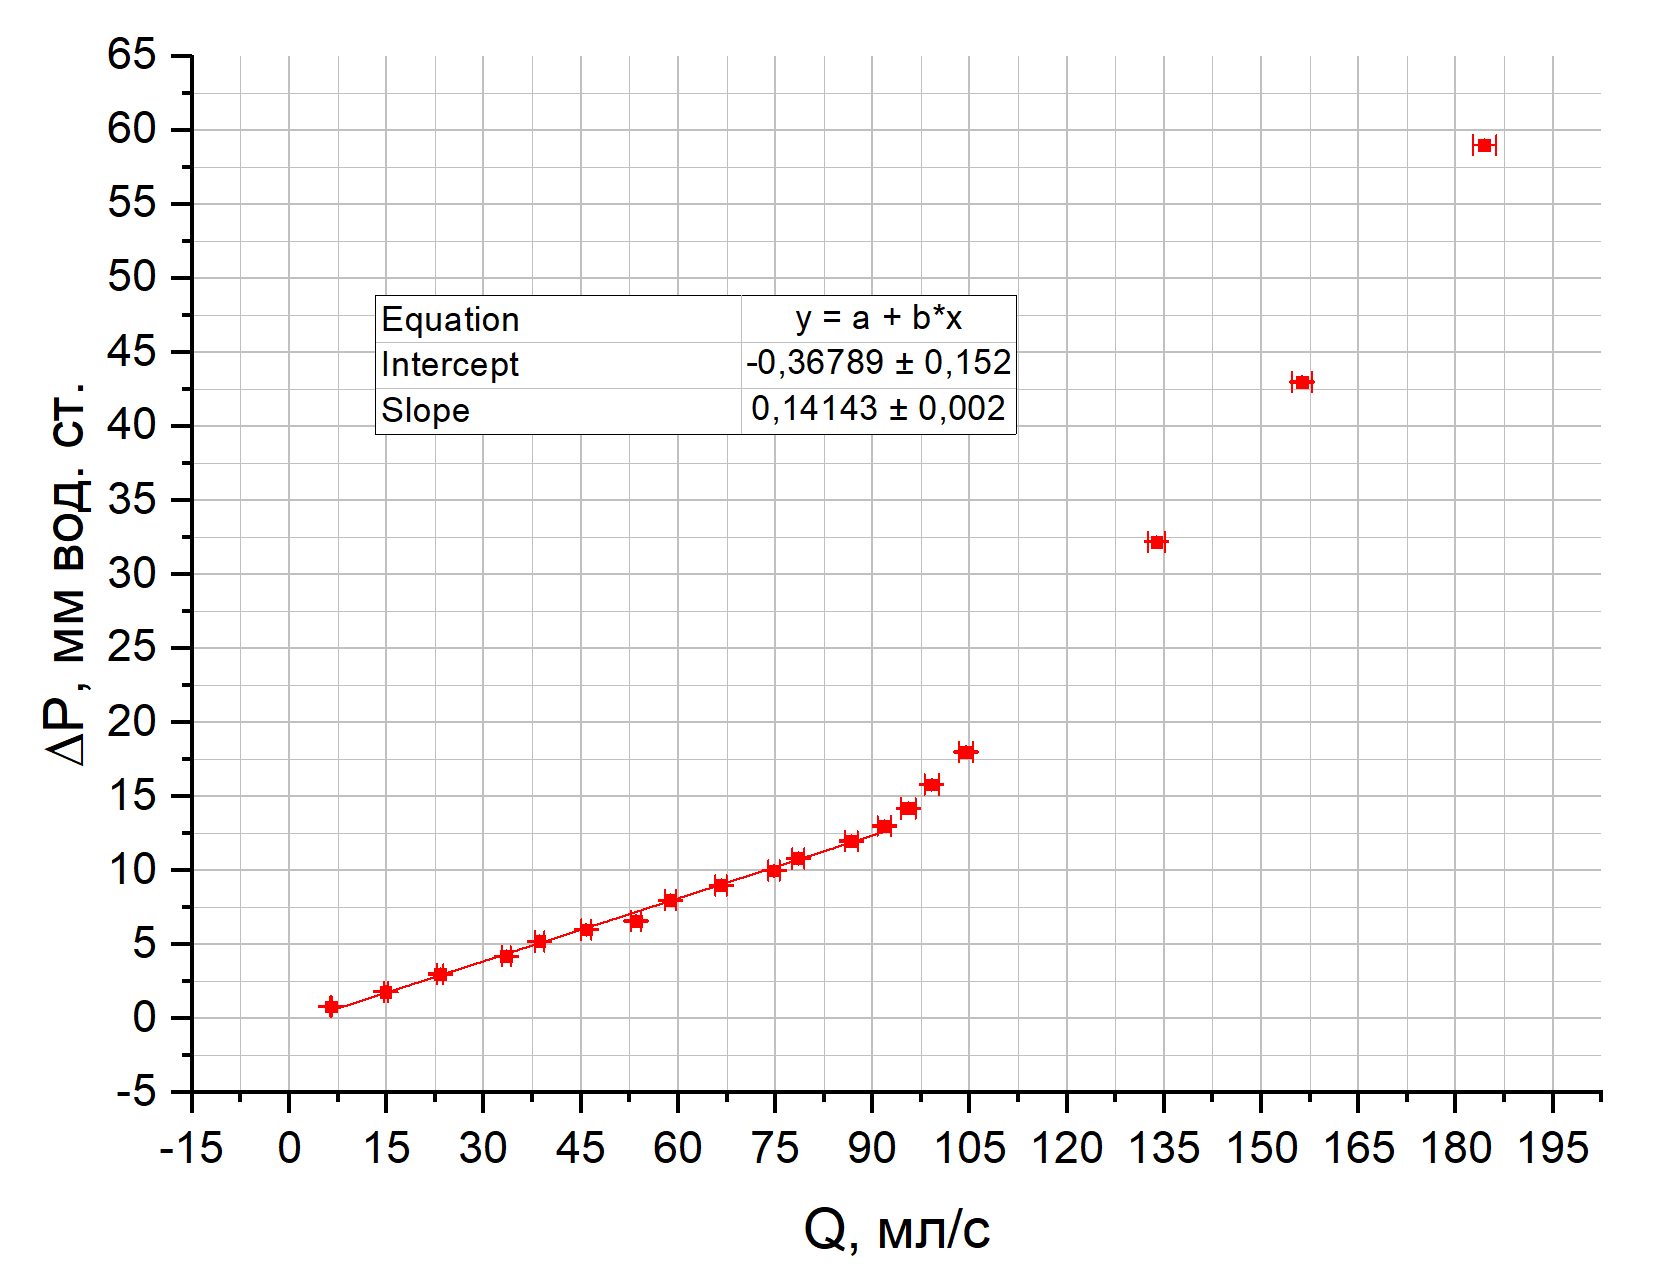
\includegraphics[width=0.85\linewidth]{5}
	\end{center}
\caption{График зависимости разности давления $\Delta P$ от расхода воздуха $Q$}
\end{figure}

\noindent Угловой коэффициент: $\alpha = (1,39\pm0,02)\frac{\text{Па} \cdot \text{с}}{\text{мл}}$

По угловому коэффициенту прямолинейного участка графика определяем вязкость воздуха $\eta$ с помощью формулы (9) $l = 50\text{см}$:
\[\eta = \frac{\pi (d_2/2)^4 \alpha}{8 l}\]
\[\eta = (19,2\pm0,5)\ \text{мкПa}\cdot \text{с}\]
\subsection{Число Рейнольдса}
Вычислим значение числа Рейнольдса 	Re для переходной области между ламинарным и турбулентным течениями. Из графика видно, что это происходит при $Q = 0,099 -0,104 \  \text{л/с} $
\[\text{Re} = \frac{Q  \rho}{\pi (d_2/2)\eta}  \]
\[ \text{Re} = 963\pm43  \]
При расходе, заведомо обеспечивающим ламинарность потока, измерим распределение давления вдоль трубки. Результаты измерений занесем в Таблицу 3.
\begin{table}[h]
	\begin{center}
	\begin{tabular}{|c|c|}
		\hline
		$\Delta P, \text{мм вод. ст.}$  &  $l, \text{см}$ \\ \hline
		39       & 130,5 \\ \hline
		25       & 80,5  \\ \hline
		14       & 40,5  \\ \hline
		5        & 10,5  \\ \hline
	\end{tabular}
\caption{Зависимость давления $\Delta P$ от длины вдоль трубки $l$}
\end{center}

\end{table}

\noindent Построим график зависимости давления от длины вдоль трубки.
\begin{figure}[h]
	\begin{center}
		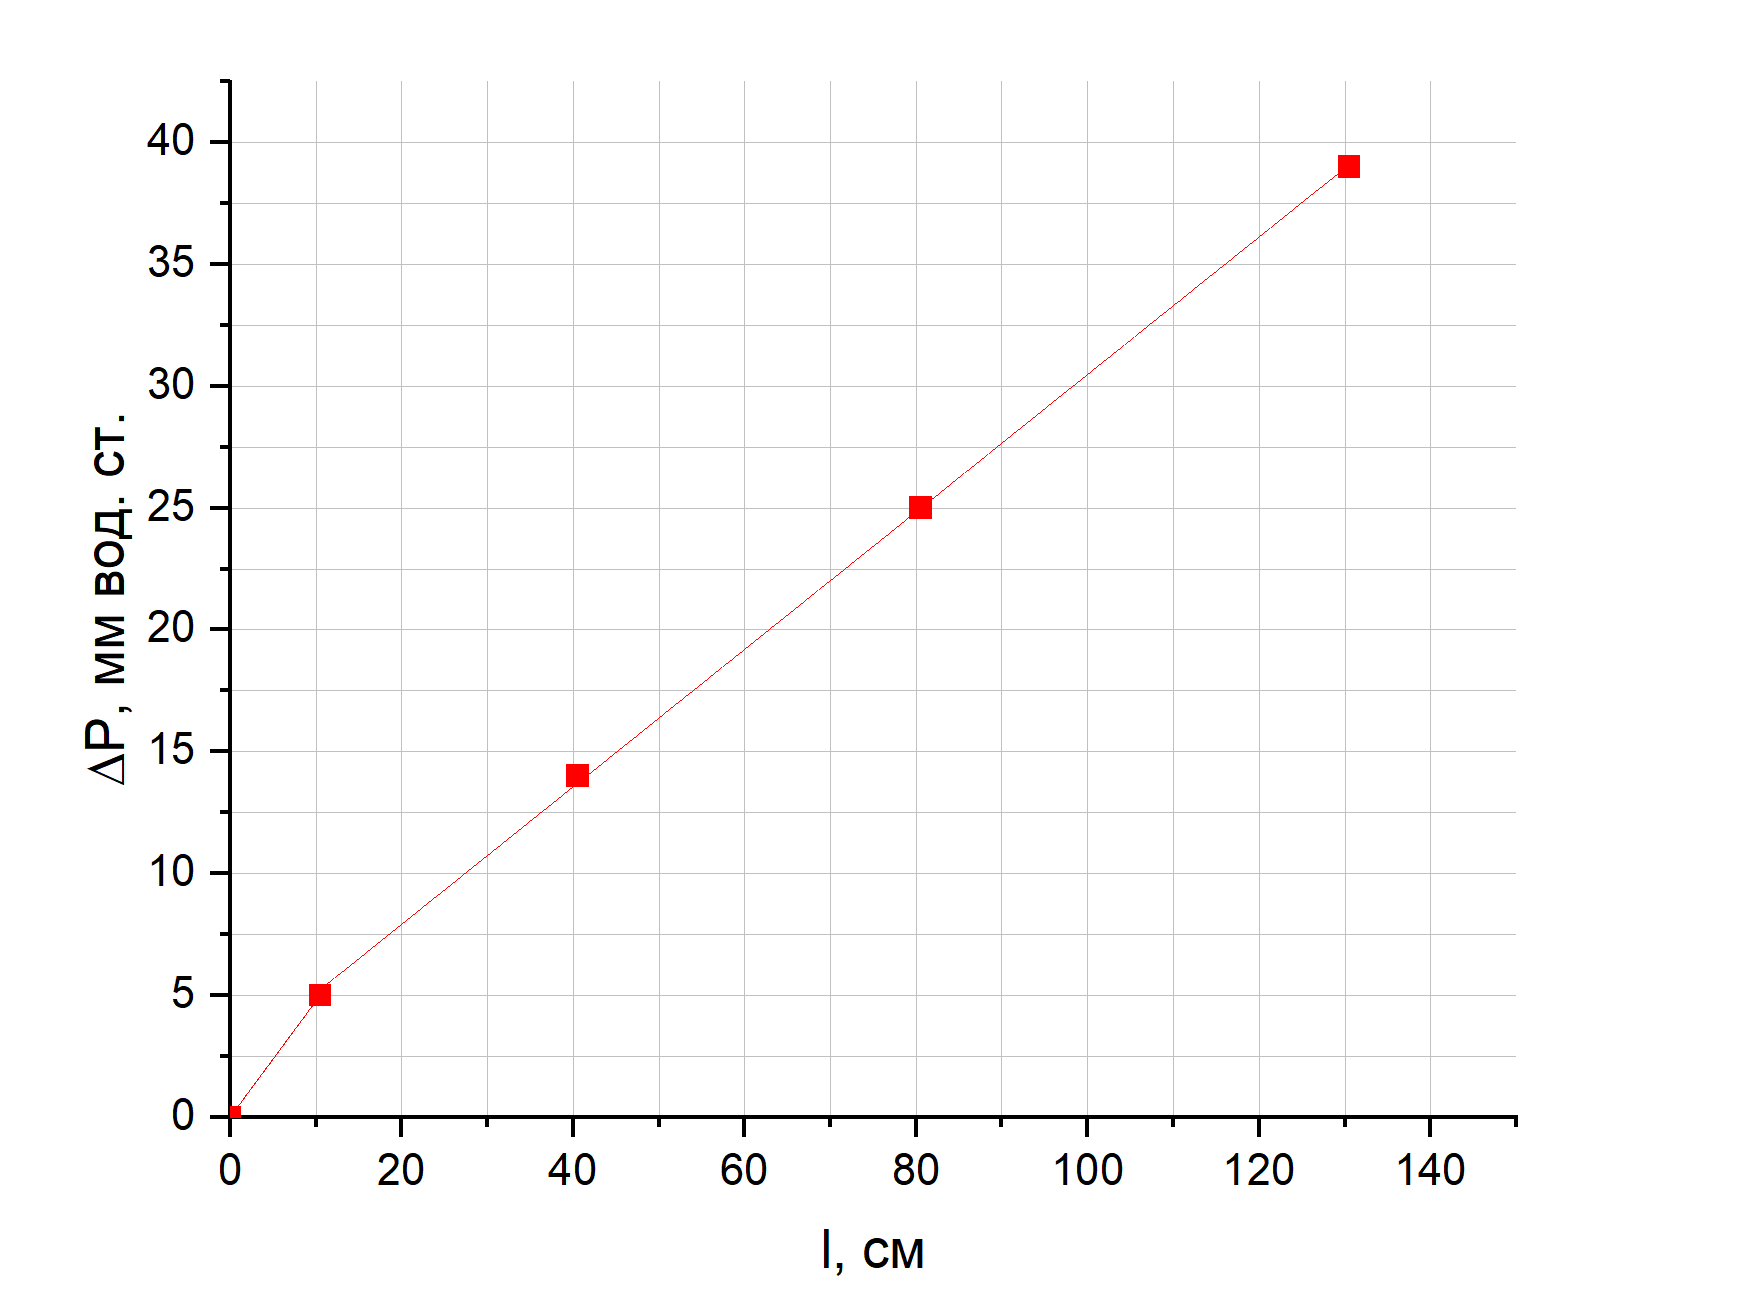
\includegraphics[width=0.55\linewidth]{7}
	\end{center}
\caption{График зависимости разности давления $\Delta P$ от длины $l$}
\end{figure}


\subsection{Показатель степени в формуле Пуазейля}
Для всех трубок на участках со сформированным течением (в конце трубок) в ламинарном режиме (Re $< 500$) снимем зависимость $Q = f(P)$. Результаты занесем в Таблицу 4.

Данные c трубки с $d = 3\text{мм}$ явно были получены с ошибками. Возможно, это связано с тем, что на конце трубки не было выхода для воздуха. Поэтому будем сравнивать значения с трубок с $d_1 = 4,1\text{мм}$ и с $d_2 = 5,8 \text{мм}$. Внесем в Таблицу 5 интересующие нас значения для определения показателя в формуле Пуазейля. Построим график зависимости показателя степени от отношения логарифмов:
\[\frac{\ln \frac{\Delta P_2}{Q_2}\frac{Q_1 }{\Delta P_1} \frac{l_1}{l_2}}{\ln \frac{d_1}{d_2}} \] 
\begin{table}[h]
	\begin{center}
	\begin{tabular}{|c|c|m{0.12\linewidth}|c|c|c|m{0.15\linewidth}|}
		\hline
		$l, \text{см} $ & $d, \text{мм}$ & $\Delta P,$ $\text{мм вод. ст.}$ & $\Delta V, \text{л}$ & $\Delta t, \text{с}$ & $Q, \text{л/с}$ & $\Delta P/ Q,$ $\text{мм вод. ст.}\cdot \text{с}/\text{л}$ \\ \hline
		\multirow{4}{*}{30} & \multirow{4}{*}{3}   & \multicolumn{1}{|c|}{2}   & 1   & 50,69 & 0,020 & \multicolumn{1}{|c|}{101,380} \\ \cline{3-7}
		&     &  \multicolumn{1}{|c|}{3,4} & 1,1 & 32,84 & 0,033 & \multicolumn{1}{|c|}{101,505} \\ \cline{3-7}
		&     &  \multicolumn{1}{|c|}{5}   & 1,5 & 32,31 & 0,046 & \multicolumn{1}{|c|}{107,700} \\ \cline{3-7}
		&     &  \multicolumn{1}{|c|}{2,8} & 1   & 36,69 & 0,027 & \multicolumn{1}{|c|}{102,732} \\ \hline
		\multirow{8}{*}{50} & \multirow{8}{*}{5,8} &  \multicolumn{1}{|c|}{3,8} & 4   & 33,87 & 0,118 & \multicolumn{1}{|c|}{32,177}  \\ \cline{3-7}
		&     &  \multicolumn{1}{|c|}{6}   & 5   & 33,03 & 0,151 & \multicolumn{1}{|c|}{39,636}  \\ \cline{3-7}
		&     &  \multicolumn{1}{|c|}{5,2} & 4,5 & 31,34 & 0,144 & \multicolumn{1}{|c|}{36,215}  \\ \cline{3-7}
		&     &  \multicolumn{1}{|c|}{4,2} & 4   & 31,37 & 0,128 & \multicolumn{1}{|c|}{32,939}  \\\cline{3-7}
		&     &  \multicolumn{1}{|c|}{8}   & 5,5 & 33,34 & 0,165 & \multicolumn{1}{|c|}{48,495}  \\ \cline{3-7}
		&     &  \multicolumn{1}{|c|}{3}   & 3   & 32,19 & 0,093 & \multicolumn{1}{|c|}{32,190}  \\ \cline{3-7}
		&     &  \multicolumn{1}{|c|}{2}   & 2   & 31,22 & 0,064 & \multicolumn{1}{|c|}{31,220}  \\ \hline
	\end{tabular}
\end{center}
\caption{Зависимость расхода воздуха $Q$ от разности давлений $\Delta P$}
\end{table}
\renewcommand\arraystretch{1.5}
\begin{table}[h]
	\begin{center}
	\begin{tabular}{|c|c|c|}
		\hline
		$\ln(d_1/d_2)$   &$\ln \frac{\Delta P_2}{Q_2}\frac{Q_1 }{\Delta P_1} \frac{l_1}{l_2}$  & $n$ \\ \hline
		-0,35 & -1,36 & 3,92  \\ \hline
		-0,35 & -1,12 & 3,22  \\ \hline
		-0,35 & -1,27 & 3,66  \\ \hline
		-0,35 & -1,34 & 3,86  \\ \hline
		-0,35 & -1,40 & 4,05  \\ \hline
		-0,35 & -1,38 & 3,96  \\ \hline
	\end{tabular}
\end{center}
\caption{Данные для определения показателя степени в формуле Пуазейля}
\end{table}
\newpage
\begin{figure}[h]
	\begin{center}
		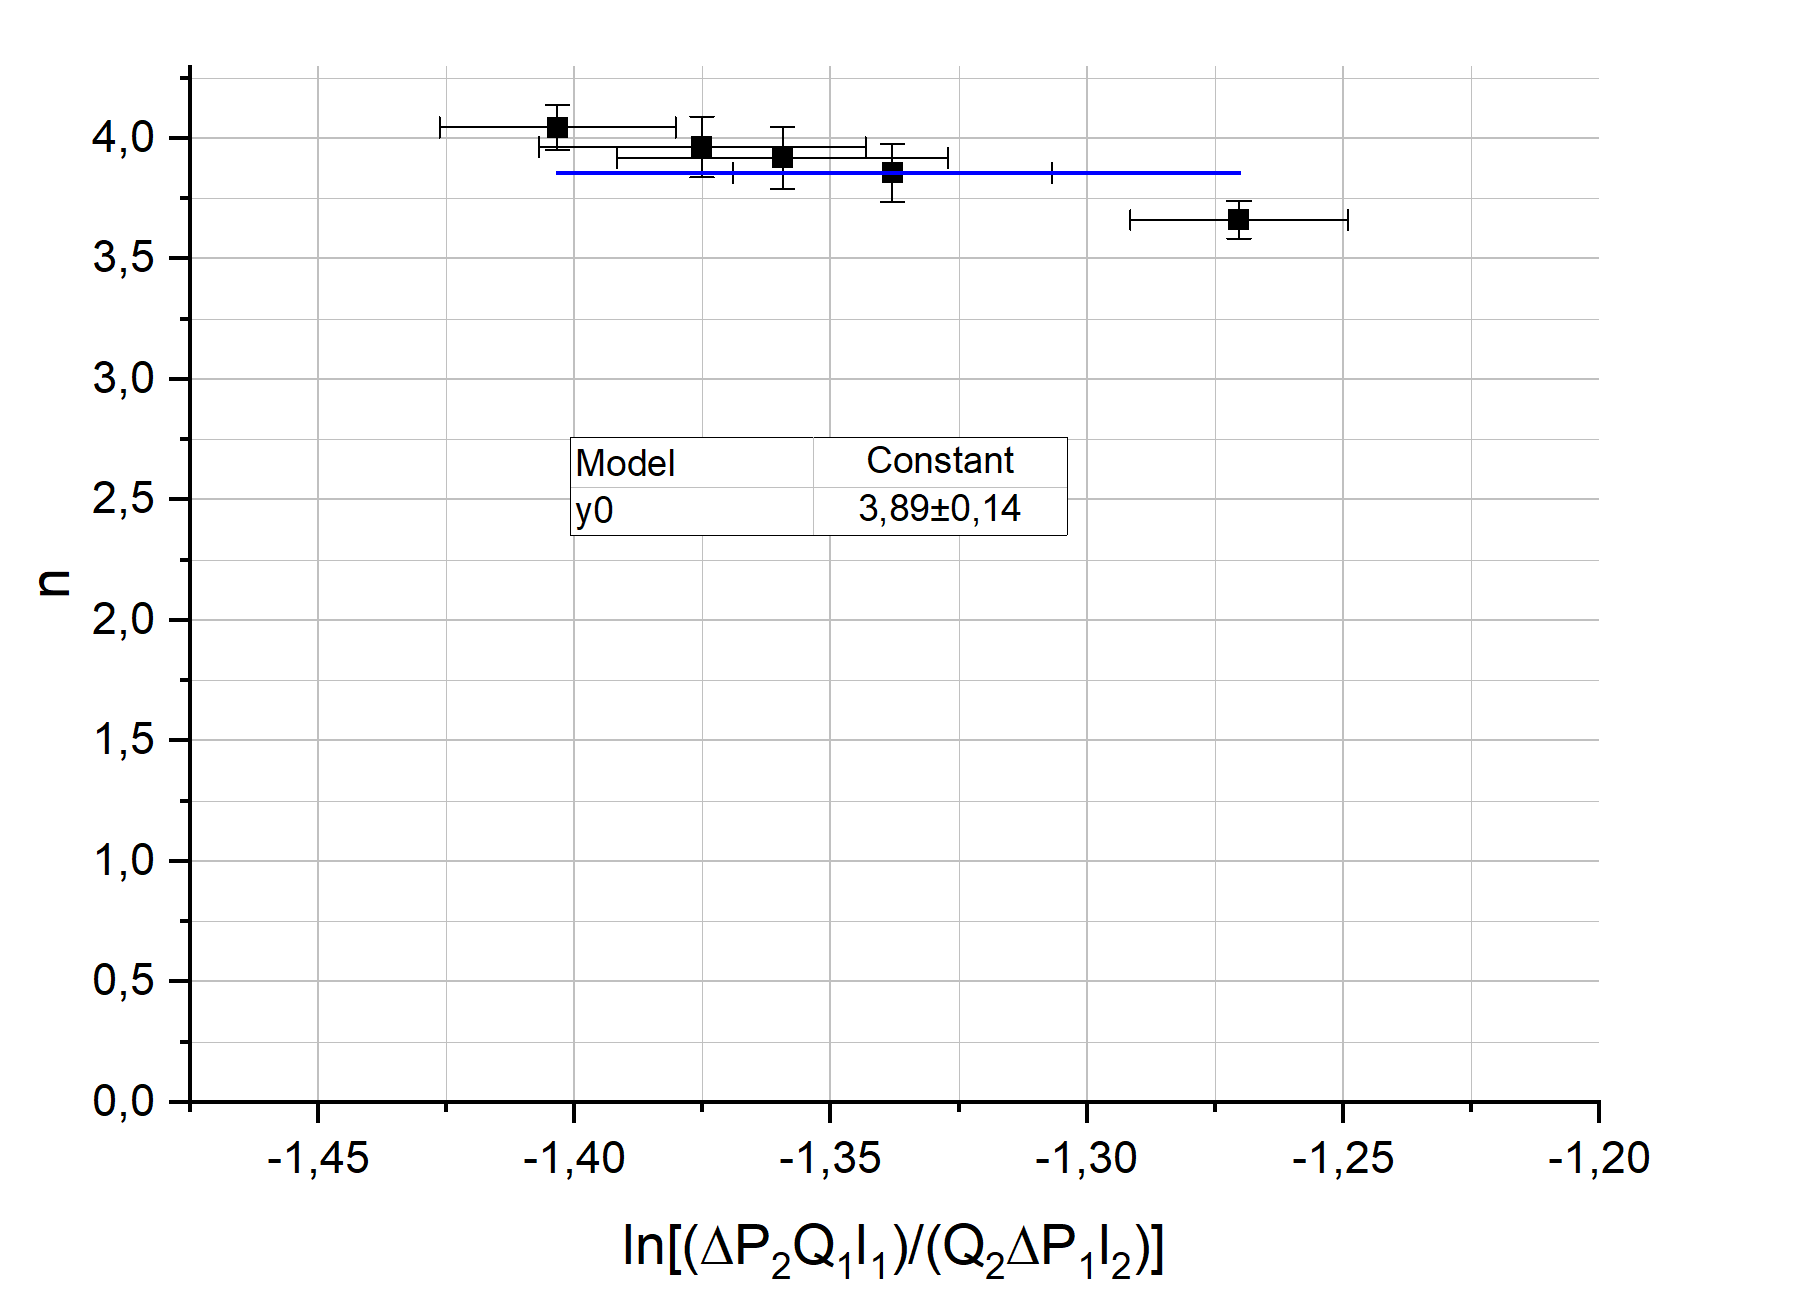
\includegraphics[width=0.7\linewidth]{6}
	\end{center}
	\caption{График зависимости показателя степени в формуле Пуазейля $n$ от $\ln \frac{\Delta P_2}{Q_2}\frac{Q_1 }{\Delta P_1} \frac{l_1}{l_2}$ }
\end{figure}
По графику получаем коэффициент $n = 3,89\pm0,14$
\section{Обсуждение результатов и выводы}
\noindent В работе эксперементально получен коэффициент вязкости воздуха
\[\eta = (19,2\pm0,5) \text{мкПа} \cdot \text{с}\]
Что практически совпадает с табличным значением вязкости при $25^\circ C$
\[\eta_{\text{табл}} = 18,4\ \text{мкПа} \cdot \text{с}\]
Было посчитано число Рейнольдса для переходной областью между ламинарным и турбулентным течением
\[\text{Re} = 963\pm43\]
Значение совпадает с теоритическим.
Была проведена оценка длины участка, на котором происходит установление потока. Исходя из графика на Рис. 6 видно, что значение полученное по формуле (11) $a = 41\ \text{см}$ обеспечивает формирование ламинарного потока.

Было получено значение степени радиуса трубы в формуле Пуазейля:
\[n = 3,9\pm0,1\]
Значение в пределах погрешности совпадает с теоритическим.

\renewcommand{\theenumii}{\asbuk{enumii}} 
\begin{enumerate}
	\item alskfja;k
	\begin{enumerate}
		\item kladfja
		\item lskjf
		\item sldkjf
		\begin{enumerate}
			\item lkfja;lfj
		\end{enumerate}
	\end{enumerate}
\end{enumerate}
\end{document} % конец документа

	